%%%% ijcai20.tex

\typeout{IJCAI--PRICAI--20 Instructions for Authors}

% These are the instructions for authors for IJCAI-20.

\documentclass{article}
\pdfpagewidth=8.5in
\pdfpageheight=11in
% The file ijcai20.sty is NOT the same than previous years'
\usepackage{ijcai20}

% Use the postscript times font!
\usepackage{times}
\usepackage{soul}
\usepackage{url}
\usepackage{hyperref}
\usepackage[utf8]{inputenc}
\usepackage[small]{caption}
\usepackage{graphicx}
% \usepackage[dvipdfmx]{color}
\usepackage{amsmath}
\usepackage{amsthm}
\usepackage{booktabs}
\usepackage{algorithm}
\usepackage{algorithmic}
\urlstyle{same}

% the following package is optional:
%\usepackage{latexsym} 

% See https://www.overleaf.com/learn/latex/theorems_and_proofs
% for a nice explanation of how to define new theorems, but keep
% in mind that the amsthm package is already included in this
% template and that you must *not* alter the styling.
\newtheorem{example}{Example}
\newtheorem{theorem}{Theorem}

% Following comment is from ijcai97-submit.tex:
% The preparation of these files was supported by Schlumberger Palo Alto
% Research, AT\&T Bell Laboratories, and Morgan Kaufmann Publishers.
% Shirley Jowell, of Morgan Kaufmann Publishers, and Peter F.
% Patel-Schneider, of AT\&T Bell Laboratories collaborated on their
% preparation.

% These instructions can be modified and used in other conferences as long
% as credit to the authors and supporting agencies is retained, this notice
% is not changed, and further modification or reuse is not restricted.
% Neither Shirley Jowell nor Peter F. Patel-Schneider can be listed as
% contacts for providing assistance without their prior permission.

% To use for other conferences, change references to files and the
% conference appropriate and use other authors, contacts, publishers, and
% organizations.
% Also change the deadline and address for returning papers and the length and
% page charge instructions.
% Put where the files are available in the appropriate places.

\title{IJCAI--PRICAI--20 Formatting Instructions}

% Single author syntax
\author{
    Christian Bessiere
    \affiliations
    CNRS, University of Montpellier, France
    \emails
    pcchair@ijcai20.org
}

% Multiple author syntax (remove the single-author syntax above and the \iffalse ... \fi here)
% Check the ijcai20-multiauthor.tex file for detailed instructions
\iffalse
\author{
First Author$^1$
\and
Second Author$^2$\and
Third Author$^{2,3}$\And
Fourth Author$^4$
\affiliations
$^1$First Affiliation\\
$^2$Second Affiliation\\
$^3$Third Affiliation\\
$^4$Fourth Affiliation
\emails
\{first, second\}@example.com,
third@other.example.com,
fourth@example.com
}
\fi

\begin{document}

\maketitle

\begin{abstract}
  The {\it IJCAI--PRICAI--20 Proceedings} will be printed from electronic
  manuscripts submitted by the authors. The electronic manuscript will
  also be included in the online version of the proceedings. This paper
  provides the style instructions.
\end{abstract}

\section{Introduction}
    \begin{figure}
        % \overfullrule=2cm
        \begin{center}
            % 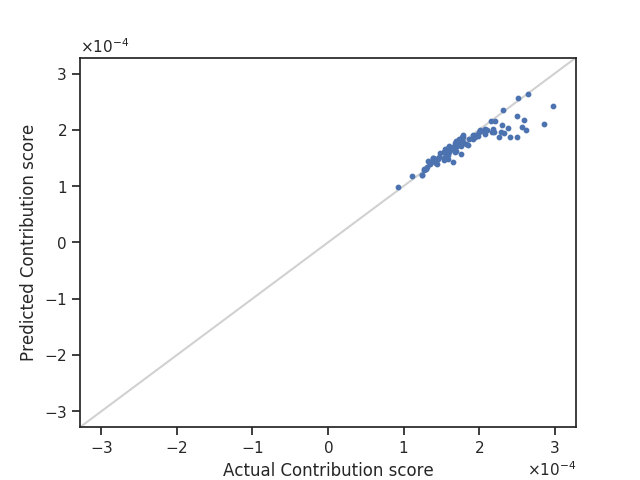
\includegraphics[width=6cm]{./media/loss_error_010.png}
            \includegraphics[width=6cm]{cifar10_ae.jpg}
            \caption{Counterfactual SGD and SGD-Influence}
            % \label{fig:error}
        \end{center}
    \end{figure}
The {\it IJCAI--20 Proceedings} will be printed from electronic
manuscripts submitted by the authors. These must be PDF ({\em Portable
Document Format}) files formatted for 8-1/2$''$ $\times$ 11$''$ paper.

\subsection{Length of Papers}

All paper {\em submissions} must have a maximum of six pages, plus at most one for references. The seventh page cannot contain {\bf anything} other than references.

The length rules may change for final camera-ready versions of accepted papers and will differ between tracks. Some tracks may include only references in the last page, whereas others allow for any content in all pages. Similarly, some tracks allow you to buy a few extra pages should you want to, whereas others don't.

If your paper is accepted, please carefully read the notifications you receive, and check the proceedings submission information website\footnote{\url{https://proceedings.ijcai.org/info}} to know how many pages you can finally use. That website holds the most up-to-date information regarding paper length limits at all times. Please notice that if your track allows for a special references-only page, the {\bf references-only page(s) cannot contain anything else than references} (i.e.: do not write your acknowledgments on that page or you will be charged for it).

\subsection{Word Processing Software}

As detailed below, IJCAI has prepared and made available a set of
\LaTeX{} macros and a Microsoft Word template for use in formatting
your paper. If you are using some other word processing software, please follow the format instructions given below and ensure that your final paper looks as much like this sample as possible.

\section{Style and Format}

\LaTeX{} and Word style files that implement these instructions
can be retrieved electronically. (See Appendix~\ref{stylefiles} for
instructions on how to obtain these files.)

\subsection{Layout}


Print manuscripts two columns to a page, in the manner in which these
instructions are printed. The exact dimensions for pages are:
\begin{itemize}
\item left and right margins: .75$''$
\item column width: 3.375$''$
\item gap between columns: .25$''$
\item top margin---first page: 1.375$''$
\item top margin---other pages: .75$''$
\item bottom margin: 1.25$''$
\item column height---first page: 6.625$''$
\item column height---other pages: 9$''$
\end{itemize}

All measurements assume an 8-1/2$''$ $\times$ 11$''$ page size. For
A4-size paper, use the given top and left margins, column width,
height, and gap, and modify the bottom and right margins as necessary.

\subsection{Format of Electronic Manuscript}

For the production of the electronic manuscript, you must use Adobe's
{\em Portable Document Format} (PDF). A PDF file can be generated, for
instance, on Unix systems using {\tt ps2pdf} or on Windows systems
using Adobe's Distiller. There is also a website with free software
and conversion services: \url{http://www.ps2pdf.com}. For reasons of
uniformity, use of Adobe's {\em Times Roman} font is strongly suggested. 
In \LaTeX2e{} this is accomplished by writing
\begin{quote} 
\mbox{\tt $\backslash$usepackage\{times\}}
\end{quote}
in the preamble.\footnote{You may want also to use the package {\tt
latexsym}, which defines all symbols known from the old \LaTeX{}
version.}

Additionally, it is of utmost importance to specify the {\bf
letter} format (corresponding to 8-1/2$''$ $\times$ 11$''$) when
formatting the paper. When working with {\tt dvips}, for instance, one
should specify {\tt -t letter}.

\subsection{Title and Author Information}

Center the title on the entire width of the page in a 14-point bold
font. The title must be capitalized using Title Case. Below it, center author name(s) in 12-point bold font. On the following line(s) place the affiliations, each affiliation on its own line using 12-point regular font. Matching between authors and affiliations can be done using numeric superindices. Optionally, a comma-separated list of email addresses follows the affiliation(s) line(s), using 12-point regular font.

\subsubsection{Blind Review}

In order to make blind reviewing possible, authors must omit their
names and affiliations when submitting the paper for review. In place
of names and affiliations, provide a list of content areas. When
referring to one's own work, use the third person rather than the
first person. For example, say, ``Previously,
Gottlob~\shortcite{gottlob:nonmon} has shown that\ldots'', rather
than, ``In our previous work~\cite{gottlob:nonmon}, we have shown
that\ldots'' Try to avoid including any information in the body of the
paper or references that would identify the authors or their
institutions. Such information can be added to the final camera-ready
version for publication.

\subsection{Abstract}

Place the abstract at the beginning of the first column 3$''$ from the
top of the page, unless that does not leave enough room for the title
and author information. Use a slightly smaller width than in the body
of the paper. Head the abstract with ``Abstract'' centered above the
body of the abstract in a 12-point bold font. The body of the abstract
should be in the same font as the body of the paper.

The abstract should be a concise, one-paragraph summary describing the
general thesis and conclusion of your paper. A reader should be able
to learn the purpose of the paper and the reason for its importance
from the abstract. The abstract should be no more than 200 words long.

\subsection{Text}

The main body of the text immediately follows the abstract. Use
10-point type in a clear, readable font with 1-point leading (10 on
11).

Indent when starting a new paragraph, except after major headings.

\subsection{Headings and Sections}

When necessary, headings should be used to separate major sections of
your paper. (These instructions use many headings to demonstrate their
appearance; your paper should have fewer headings.). All headings should be capitalized using Title Case.

\subsubsection{Section Headings}

Print section headings in 12-point bold type in the style shown in
these instructions. Leave a blank space of approximately 10 points
above and 4 points below section headings.  Number sections with
arabic numerals.

\subsubsection{Subsection Headings}

Print subsection headings in 11-point bold type. Leave a blank space
of approximately 8 points above and 3 points below subsection
headings. Number subsections with the section number and the
subsection number (in arabic numerals) separated by a
period.

\subsubsection{Subsubsection Headings}

Print subsubsection headings in 10-point bold type. Leave a blank
space of approximately 6 points above subsubsection headings. Do not
number subsubsections.

\paragraph{Titled paragraphs.} You should use titled paragraphs if and 
only if the title covers exactly one paragraph. Such paragraphs should be
separated from the preceding content by at least 3pt, and no more than
6pt. The title should be in 10pt bold font and ended with a period. 
After that, a 1em horizontal space should follow the title before 
the paragraph's text.

In \LaTeX{} titled paragraphs should be typeset using
\begin{quote}
{\tt \textbackslash{}paragraph\{Title.\} text} .
\end{quote}

\subsubsection{Acknowledgements}

You may include an unnumbered acknowledgments section, including
acknowledgments of help from colleagues, financial support, and
permission to publish. If present, acknowledgements must be in a dedicated,
unnumbered section appearing after all regular sections but before any
appendices or references.

Use 
\begin{quote}
    {\tt \textbackslash{}section*\{Acknowledgements\}})
\end{quote}
to typeset the acknowledgements section in \LaTeX{}.

\subsubsection{Appendices}

Any appendices directly follow the text and look like sections, except
that they are numbered with capital letters instead of arabic
numerals. See this document for an example.

\subsubsection{References}

The references section is headed ``References'', printed in the same
style as a section heading but without a number. A sample list of
references is given at the end of these instructions. Use a consistent
format for references. The reference list should not include unpublished
work.

\subsection{Citations}

Citations within the text should include the author's last name and
the year of publication, for example~\cite{gottlob:nonmon}.  Append
lowercase letters to the year in cases of ambiguity.  Treat multiple
authors as in the following examples:~\cite{abelson-et-al:scheme}
or~\cite{bgf:Lixto} (for more than two authors) and
\cite{brachman-schmolze:kl-one} (for two authors).  If the author
portion of a citation is obvious, omit it, e.g.,
Nebel~\shortcite{nebel:jair-2000}.  Collapse multiple citations as
follows:~\cite{gls:hypertrees,levesque:functional-foundations}.
\nocite{abelson-et-al:scheme}
\nocite{bgf:Lixto}
\nocite{brachman-schmolze:kl-one}
\nocite{gottlob:nonmon}
\nocite{gls:hypertrees}
\nocite{levesque:functional-foundations}
\nocite{levesque:belief}
\nocite{nebel:jair-2000}

\subsection{Footnotes}

Place footnotes at the bottom of the page in a 9-point font.  Refer to
them with superscript numbers.\footnote{This is how your footnotes
should appear.} Separate them from the text by a short
line.\footnote{Note the line separating these footnotes from the
text.} Avoid footnotes as much as possible; they interrupt the flow of
the text.

\section{Illustrations}

Place all illustrations (figures, drawings, tables, and photographs)
throughout the paper at the places where they are first discussed,
rather than at the end of the paper.

They should be floated to the top (preferred) or bottom of the page, 
unless they are an integral part 
of your narrative flow. When placed at the bottom or top of
a page, illustrations may run across both columns, but not when they
appear inline.

Illustrations must be rendered electronically or scanned and placed
directly in your document. They should be cropped outside latex, otherwise portions of the image could reappear during the post-processing of your paper. All illustrations should be understandable when printed in black and
white, albeit you can use colors to enhance them. Line weights should
be 1/2-point or thicker. Avoid screens and superimposing type on
patterns, as these effects may not reproduce well.

Number illustrations sequentially. Use references of the following
form: Figure 1, Table 2, etc. Place illustration numbers and captions
under illustrations. Leave a margin of 1/4-inch around the area
covered by the illustration and caption.  Use 9-point type for
captions, labels, and other text in illustrations. Captions should always appear below the illustration.

\section{Tables}

Tables are considered illustrations containing data. Therefore, they should also appear floated to the top (preferably) or bottom of the page, and with the captions below them.

\begin{table}
\centering
\begin{tabular}{lll}
\hline
Scenario  & $\delta$ & Runtime \\
\hline
Paris       & 0.1s  & 13.65ms     \\
Paris       & 0.2s  & 0.01ms      \\
New York    & 0.1s  & 92.50ms     \\
Singapore   & 0.1s  & 33.33ms     \\
Singapore   & 0.2s  & 23.01ms     \\
\hline
\end{tabular}
\caption{Latex default table}
\label{tab:plain}
\end{table}

\begin{table}
\centering
\begin{tabular}{lrr}  
\toprule
Scenario  & $\delta$ (s) & Runtime (ms) \\
\midrule
Paris       & 0.1  & 13.65      \\
            & 0.2  & 0.01       \\
New York    & 0.1  & 92.50      \\
Singapore   & 0.1  & 33.33      \\
            & 0.2  & 23.01      \\
\bottomrule
\end{tabular}
\caption{Booktabs table}
\label{tab:booktabs}
\end{table}

If you are using \LaTeX, you should use the {\tt booktabs} package, because it produces better tables than the standard ones. Compare Tables \ref{tab:plain} and~\ref{tab:booktabs}. The latter is clearly more readable for three reasons:

\begin{enumerate}
    \item The styling is better thanks to using the {\tt booktabs} rulers instead of the default ones.
    \item Numeric columns are right-aligned, making it easier to compare the numbers. Make sure to also right-align the corresponding headers, and to use the same precision for all numbers.
    \item We avoid unnecessary repetition, both between lines (no need to repeat the scenario name in this case) as well as in the content (units can be shown in the column header).
\end{enumerate}

\section{Formulas}

IJCAI's two-column format makes it difficult to typeset long formulas. A usual temptation is to reduce the size of the formula by using the {\tt small} or {\tt tiny} sizes. This doesn't work correctly with the current \LaTeX{} versions, breaking the line spacing of the preceding paragraphs and title, as well as the equation number sizes. The following equation demonstrates the effects (notice that this entire paragraph looks badly formatted):
%
\begin{tiny}
\begin{equation}
    x = \prod_{i=1}^n \sum_{j=1}^n j_i + \prod_{i=1}^n \sum_{j=1}^n i_j + \prod_{i=1}^n \sum_{j=1}^n j_i + \prod_{i=1}^n \sum_{j=1}^n i_j + \prod_{i=1}^n \sum_{j=1}^n j_i
\end{equation}
\end{tiny}%

Reducing formula sizes this way is strictly forbidden. We {\bf strongly} recommend authors to split formulas in multiple lines when they don't fit in a single line. This is the easiest approach to typeset those formulas and provides the most readable output%
%
\begin{align}
    x =& \prod_{i=1}^n \sum_{j=1}^n j_i + \prod_{i=1}^n \sum_{j=1}^n i_j + \prod_{i=1}^n \sum_{j=1}^n j_i + \prod_{i=1}^n \sum_{j=1}^n i_j + \nonumber\\
    + & \prod_{i=1}^n \sum_{j=1}^n j_i
\end{align}%

If a line is just slightly longer than the column width, you may use the {\tt resizebox} environment on that equation. The result looks better and doesn't interfere with the paragraph's line spacing: %
\begin{equation}
\resizebox{.91\linewidth}{!}{$
    \displaystyle
    x = \prod_{i=1}^n \sum_{j=1}^n j_i + \prod_{i=1}^n \sum_{j=1}^n i_j + \prod_{i=1}^n \sum_{j=1}^n j_i + \prod_{i=1}^n \sum_{j=1}^n i_j + \prod_{i=1}^n \sum_{j=1}^n j_i
$}
\end{equation}%

This last solution may have to be adapted if you use different equation environments, but it can generally be made to work. Please notice that in any case:

\begin{itemize}
    \item Equation numbers must be in the same font and size than the main text (10pt).
    \item Your formula's main symbols should not be smaller than {\small small} text (9pt).
\end{itemize}

For instance, the formula
%
\begin{equation}
    \resizebox{.91\linewidth}{!}{$
    \displaystyle
    x = \prod_{i=1}^n \sum_{j=1}^n j_i + \prod_{i=1}^n \sum_{j=1}^n i_j + \prod_{i=1}^n \sum_{j=1}^n j_i + \prod_{i=1}^n \sum_{j=1}^n i_j + \prod_{i=1}^n \sum_{j=1}^n j_i + \prod_{i=1}^n \sum_{j=1}^n i_j
$}
\end{equation}
% 
would not be acceptable because the text is too small.

\section{Examples, Definitions, Theorems and Similar}

Examples, definitions, theorems, corollaries and similar must be written in their own paragraph. The paragraph must be separated by at least 2pt and no more than 5pt from the preceding and succeeding paragraphs. They must begin with the kind of item written in 10pt bold font followed by their number (e.g.: Theorem 1), optionally followed by a title/summary between parentheses in non-bold font and ended with a period. After that the main body of the item follows, written in 10 pt italics font (see below for examples). 

In \LaTeX{} We strongly recommend you to define environments for your examples, definitions, propositions, lemmas, corollaries and similar. This can be done in your \LaTeX{} preamble using \texttt{\textbackslash{newtheorem}} -- see the source of this document for examples. Numbering for these items must be global, not per-section (e.g.: Theorem 1 instead of Theorem 6.1).

\begin{example}[How to write an example]
Examples should be written using the example environment defined in this template.
\end{example}

\begin{theorem}
This is an example of an untitled theorem.
\end{theorem}

You may also include a title or description using these environments as shown in the following theorem.

\begin{theorem}[A titled theorem]
This is an example of a titled theorem.
\end{theorem}

\section{Proofs}

Proofs must be written in their own paragraph separated by at least 2pt and no more than 5pt from the preceding and succeeding paragraphs. Proof paragraphs should start with the keyword ``Proof." in 10pt italics font. After that the proof follows in regular 10pt font. At the end of the proof, an unfilled square symbol (qed) marks the end of the proof.

In \LaTeX{} proofs should be typeset using the \texttt{\textbackslash{proof}} environment.

\begin{proof}
This paragraph is an example of how a proof looks like using the \texttt{\textbackslash{proof}} environment. 
\end{proof}


\section{Algorithms and Listings}

Algorithms and listings are a special kind of figures. Like all illustrations, they should appear floated to the top (preferably) or bottom of the page. However, their caption should appear in the header, left-justified and enclosed between horizontal lines, as shown in Algorithm~\ref{alg:algorithm}. The algorithm body should be terminated with another horizontal line. It is up to the authors to decide whether to show line numbers or not, how to format comments, etc.

In \LaTeX{} algorithms may be typeset using the {\tt algorithm} and {\tt algorithmic} packages, but you can also use one of the many other packages for the task.  

\begin{algorithm}[tb]
\caption{Example algorithm}
\label{alg:algorithm}
\textbf{Input}: Your algorithm's input\\
\textbf{Parameter}: Optional list of parameters\\
\textbf{Output}: Your algorithm's output
\begin{algorithmic}[1] %[1] enables line numbers
\STATE Let $t=0$.
\WHILE{condition}
\STATE Do some action.
\IF {conditional}
\STATE Perform task A.
\ELSE
\STATE Perform task B.
\ENDIF
\ENDWHILE
\STATE \textbf{return} solution
\end{algorithmic}
\end{algorithm}

\section*{Acknowledgments}

The preparation of these instructions and the \LaTeX{} and Bib\TeX{}
files that implement them was supported by Schlumberger Palo Alto
Research, AT\&T Bell Laboratories, and Morgan Kaufmann Publishers.
Preparation of the Microsoft Word file was supported by IJCAI.  An
early version of this document was created by Shirley Jowell and Peter
F. Patel-Schneider.  It was subsequently modified by Jennifer
Ballentine and Thomas Dean, Bernhard Nebel, Daniel Pagenstecher,
Kurt Steinkraus, Toby Walsh and Carles Sierra. The current version 
has been prepared by Marc Pujol-Gonzalez and Francisco Cruz-Mencia.

\appendix

\section{\LaTeX{} and Word Style Files}\label{stylefiles}

The \LaTeX{} and Word style files are available on the IJCAI--PRICAI--20
website, \url{https://www.ijcai20.org/}.
These style files implement the formatting instructions in this
document.

The \LaTeX{} files are {\tt ijcai20.sty} and {\tt ijcai20.tex}, and
the Bib\TeX{} files are {\tt named.bst} and {\tt ijcai20.bib}. The
\LaTeX{} style file is for version 2e of \LaTeX{}, and the Bib\TeX{}
style file is for version 0.99c of Bib\TeX{} ({\em not} version
0.98i). The {\tt ijcai20.sty} style differs from the {\tt
ijcai19.sty} file used for IJCAI--19.

The Microsoft Word style file consists of a single file, {\tt
ijcai20.doc}. This template differs from the one used for
IJCAI--19.

These Microsoft Word and \LaTeX{} files contain the source of the
present document and may serve as a formatting sample.  

Further information on using these styles for the preparation of
papers for IJCAI--PRICAI--20 can be obtained by contacting {\tt
pcchair@ijcai20.org}.

%% The file named.bst is a bibliography style file for BibTeX 0.99c
\bibliographystyle{named}
\bibliography{ijcai20}

\end{document}

